\chapter{Finite element method}

\section{Bramble-Hilbert Lemma (1970)}
Bramble-Hilbert Lemma\cite{bramble1970estimation}
\includepdf[pages = -]{Papers/FEM/bramble1970estimation.pdf}


\section{Rayleigh-Ritz-Galerkin methods for dirichlet's problem using subspaces without boundary conditions (1970)}
Rayleigh-Ritz-Galerkin methods for dirichlet's problem using subspaces without boundary conditions\cite{bramble1970rayleigh}
\includepdf[pages = -]{Papers/FEM/bramble1970rayleigh.pdf}


\section{Triangular elements in the finite element method (1970)}
Triangular elements in the finite element method\cite{bramble1970triangular}
\includepdf[pages = -]{Papers/FEM/bramble1970triangular.pdf}


\section{Maximum-norm interior estimates for Ritz-Galerkin methods (1975)}
\cite{bramble1975maximum}
\includepdf[pages = -]{Papers/FEM/bramble1975maximum.pdf}


\section{Estimates for spline projections (1976)}
Estimates for spline projections\cite{bramble1976estimates}
\includepdf[pages = -]{Papers/FEM/bramble1976estimates.pdf}



\section{Single step Galerkin approximations for parabolic problems (1977)}
Single step Galerkin approximations for parabolic problems\cite{baker1977single}
\includepdf[pages = -]{Papers/FEM/baker1977single.pdf}


\section{Some convergence estimates for semidiscrete Galerkin type approximations for parabolic equations (1977)}
Some convergence estimates for semidiscrete Galerkin type approximations for parabolic equations\cite{bramble1977some}
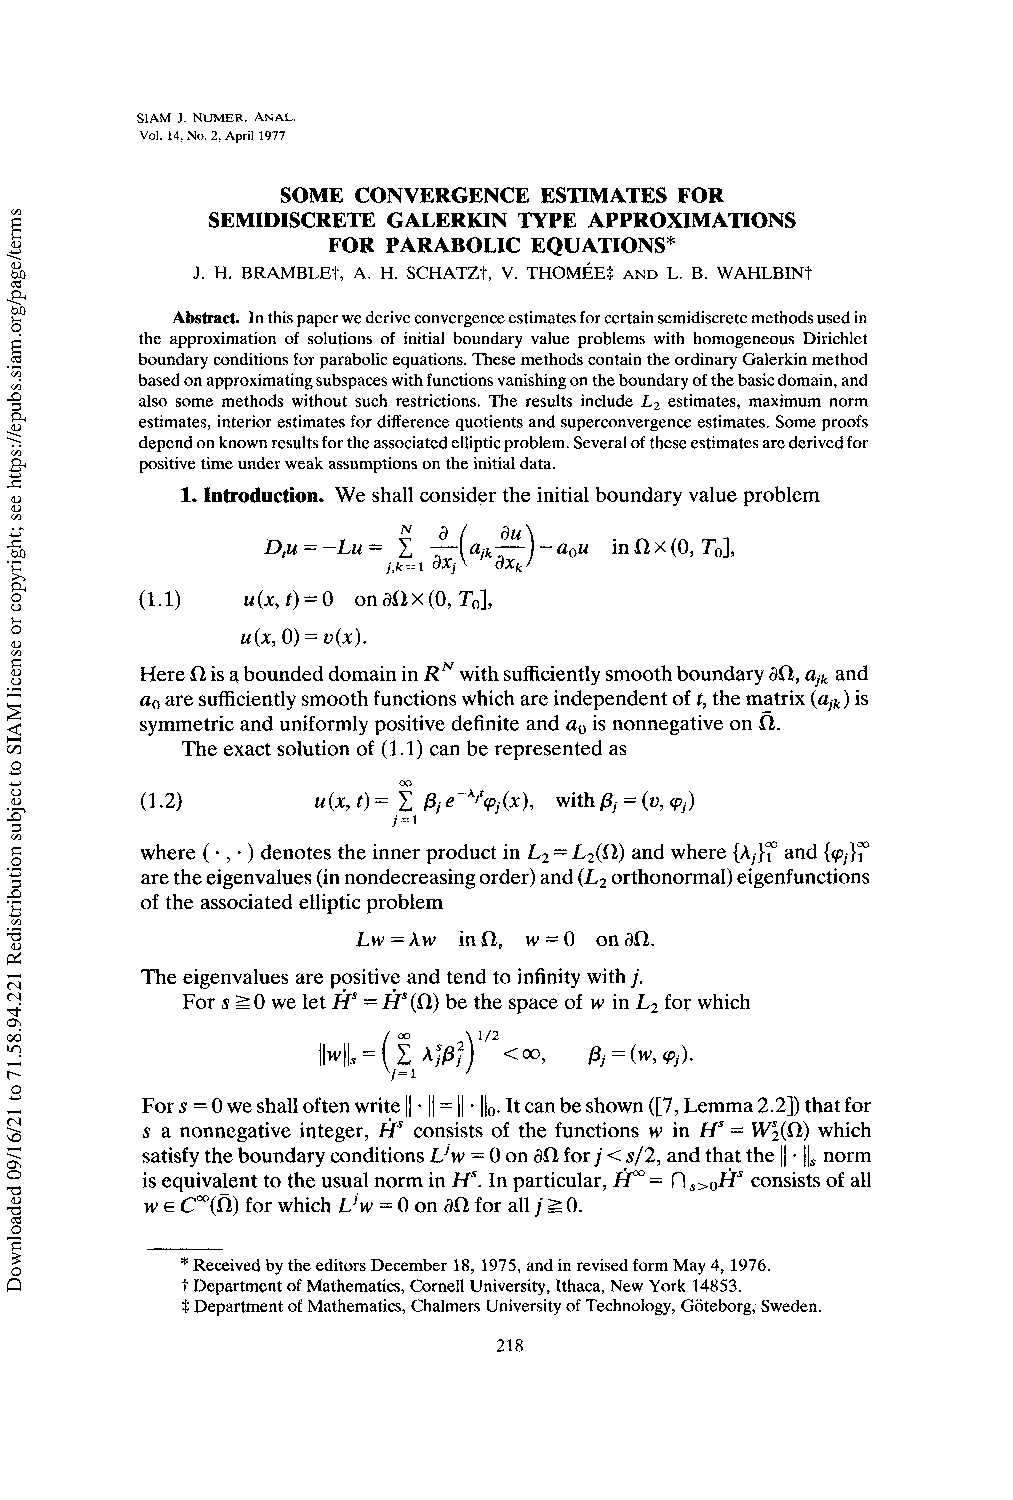
\includepdf[pages = -]{Papers/FEM/bramble1977some.pdf}


\section{Semidiscrete and single step fully discrete approximations for second order hyperbolic equations (1979)}
\cite{baker1979semidiscrete}
\includepdf[pages = -]{Papers/FEM/baker1979semidiscrete.pdf}


\section{Some estimates for a weighted $L^2$ projection (1991)}
Some estimates for a weighted $L^2$ projection\cite{bramble1991some}
\includepdf[pages = -]{Papers/FEM/bramble1991some.pdf}

\section{On variational formulations for the Stokes equations with nonstandard boundary conditions (1994)}
On variational formulations for the Stokes equations with nonstandard boundary conditions\cite{bramble1994variational}
\includepdf[pages = -]{Papers/FEM/bramble1994variational.pdf}


\section{A finite element method for interface problems in domains with smooth boundaries and interfaces (1996)}
A finite element method for interface problems in domains with smooth boundaries and interfaces\cite{bramble1996finite}
\includepdf[pages = -]{Papers/FEM/bramble1996finite.pdf}



\section{New interpolation results and applications to finite element methods for elliptic boundary value problems (2001)}
New interpolation results and applications to finite element methods for elliptic boundary value problems\cite{bacuta2001new}
\includepdf[pages = -]{Papers/FEM/bacuta2001new.pdf}


\section{On the stability of the L2 projection in $H^1(\Omega)$ (2002)}
On the stability of the L2 projection in $H^1(\Omega)$\cite{bramble2002stability}
\includepdf[pages = -]{Papers/FEM/bramble2002stability.pdf}

\section{A proof of the inf--sup condition for the Stokes equations on Lipschitz domains (2003)}
A proof of the inf--sup condition for the Stokes equations on Lipschitz domains\cite{bramble2003proof}
\includepdf[pages = -]{Papers/FEM/bramble2003proof.pdf}

\section{Using finite element tools in proving shift theorems for elliptic boundary value problems (2003)}
Using finite element tools in proving shift theorems for elliptic boundary value problems\cite{bacuta2003using}
\includepdf[pages = -]{Papers/FEM/bacuta2003using.pdf}


\section{Super-convergence}

\subsection{Higher order local accuracy by averaging in the finite element method (1977)}
Higher order local accuracy by averaging in the finite element method\cite{bramble1977higher}
\includepdf[pages = -]{Papers/FEM/bramble1977higher.pdf}

\subsection{A local post-processing technique for improving the accuracy in mixed finite-element approximations (1989)}
A local post-processing technique for improving the accuracy in mixed finite-element approximations\cite{bramble1989local}
\includepdf[pages = -]{Papers/FEM/bramble1989local.pdf}


%\subsection{A local post-processing technique for improving the accuracy in mixed finite-element approximations}
%A local post-processing technique for improving the accuracy in mixed finite-element approximations \cite{bramble1989local}.
%\includepdf[pages = -]{Papers/FEM/bramble1989local.pdf}

%\subsection{Higher order local accuracy by averaging in the finite element method}
%Higher order local accuracy by averaging in the finite element method \cite{bramble1977higher}.
%\includepdf[pages = -]{Papers/FEM/bramble1977higher.pdf}


